% ============================== CHAPTER 4 ===================================
\chapter{Project Planning}
\label{ch:planning}

Planning a machine learning systems project differs from planning conventional
software in one decisive respect: several tasks have durations that cannot be
known until they are attempted, and some have outcomes that determine which
tasks follow. Teacher distillation over half a million sentences takes as long
as it takes; a student either converges or collapses, and a collapse adds an
unplanned diagnostic and retraining cycle. The plan described here was therefore
built around milestones with explicit evidence requirements rather than around
fixed-duration activities, and it carried deliberate slack on the training
tasks.

This chapter presents the work breakdown structure, the schedule as a Gantt
chart across both project phases, a PERT analysis with the critical path, the
risk register with the mitigations actually applied, and the division of
responsibility within the team.

\section{Project Planning and Scheduling}
\label{sec:planning}

\subsection{Work Breakdown Structure}
\label{subsec:wbs}

The project decomposes into nine engineering milestones, M0 through M8, followed
by a hardening and delivery milestone. Each milestone is a single commit with a
defined completion criterion, so that progress is verifiable rather than
self-reported. Table~\ref{tab:wbs} gives the breakdown together with the
evidence required to close each item.

\begin{longtable}{@{}p{1.1cm} L{3.5cm} L{5.4cm} L{4.1cm}@{}}
\caption{Work breakdown structure with completion evidence}
\label{tab:wbs}\\
\toprule
\rowcolor{headblue}
\textbf{ID} & \textbf{Task} & \textbf{Description} & \textbf{Completion evidence} \\
\midrule
\endfirsthead
\multicolumn{4}{c}{\textit{Table \thetable{} --- continued from previous page}}\\
\toprule
\rowcolor{headblue}
\textbf{ID} & \textbf{Task} & \textbf{Description} & \textbf{Completion evidence} \\
\midrule
\endhead
\midrule
\multicolumn{4}{r}{\textit{continued on next page}}\\
\endfoot
\bottomrule
\endlastfoot

M0 & Scaffold & Package layout, four core data objects, YAML configuration with the 22-language registry, CLI, passthrough stub engine & 7 tests green; CLI runs end to end \\
\rowcolor{rowgrey}
M1 & Data pipeline & Corpus loading, script normalisation, length and script filtering, deduplication, JSONL output & 50{,}000 pairs in, 49{,}520 clean pairs out, with a filter breakdown report \\
M2 & Teacher integration & IndicTrans2 behind an abstract interface; a test forbids any other module importing the teacher's dependencies & Real smoke test producing fluent candidate translations \\
\rowcolor{rowgrey}
M3 & Preference generation & Teacher $n$-best candidates plus $k$-NN retrieved neighbours, chrF ranking, pair validation & 500 entries $\rightarrow$ 3{,}494 candidates $\rightarrow$ 2{,}074 validated pairs \\
M4 & SFT and DPO training & SentencePiece tokenizer, student model, supervised fine-tuning, DPO with a frozen reference, evaluation harness & DPO measurably outperforms SFT; test enforces the reference stays frozen \\
\rowcolor{rowgrey}
M5 & Quantisation and offline inference & ONNX export, progressive INT8 and INT4 quantisation, ONNX inference engine, socket-disabling offline assertion & Size, latency and offline targets all pass \\
M6 & Interfaces & FastAPI REST service, CLI, offline PWA, mobile SDK stubs, all sharing one engine & 15 interface tests green \\
\rowcolor{rowgrey}
M7 & All-in-One KD & Temperature-sampled cross-lingual balancing with a coverage report & Mechanism proven by test \\
M8 & Elastic Weight Consolidation & Diagonal-Fisher penalty, old-task snapshot, EWC training step & Measured retention of the old task above naive fine-tuning \\
\rowcolor{rowgrey}
M9 & Hardening and delivery & Scorecard generator, benchmarks, documentation, dead-code removal & Full suite green; scorecard reports \textsc{unverified} when evidence is absent \\
\midrule
P2-A & \seqkd{} baseline and head-to-head & Distiller CLI, \texttt{-{}-train-corpus} switch, S0/S1/S2/S3 comparison & Table~\ref{tab:h1} filled \\
\rowcolor{rowgrey}
P2-B & GPU campaign & Environment fixes, resumable runners, 22 directions trained bidirectionally & 22 per-direction reports \\
P2-C & Collapse diagnosis and recovery & Root-cause the two degenerate students and retrain & Both recovered to passing ratios \\
\rowcolor{rowgrey}
P2-D & English-pivot routing & Shared router used by REST and CLI alike & Verified on Hindi--Bengali, Tamil--Telugu, Assamese--Bengali \\
P2-E & Frontend and release & Next.js client, offline PWA, public model release, quick-start documentation & Live demo; models downloadable without login \\
\rowcolor{rowgrey}
P2-F & Report and paper & This report; paper plan with filled result tables & Submitted \\

\end{longtable}

\subsection{Gantt Chart}
\label{subsec:gantt}

Figure~\ref{fig:gantt} gives the schedule. Phase~1 ran from January to
mid-August 2026 and delivered the pipeline, the empirical finding and eleven
languages. Phase~2 runs from August to the end of October 2026 and covers the
remaining languages, benchmark rescoring, edge packaging and the final report.

\begin{figure}[H]
\centering
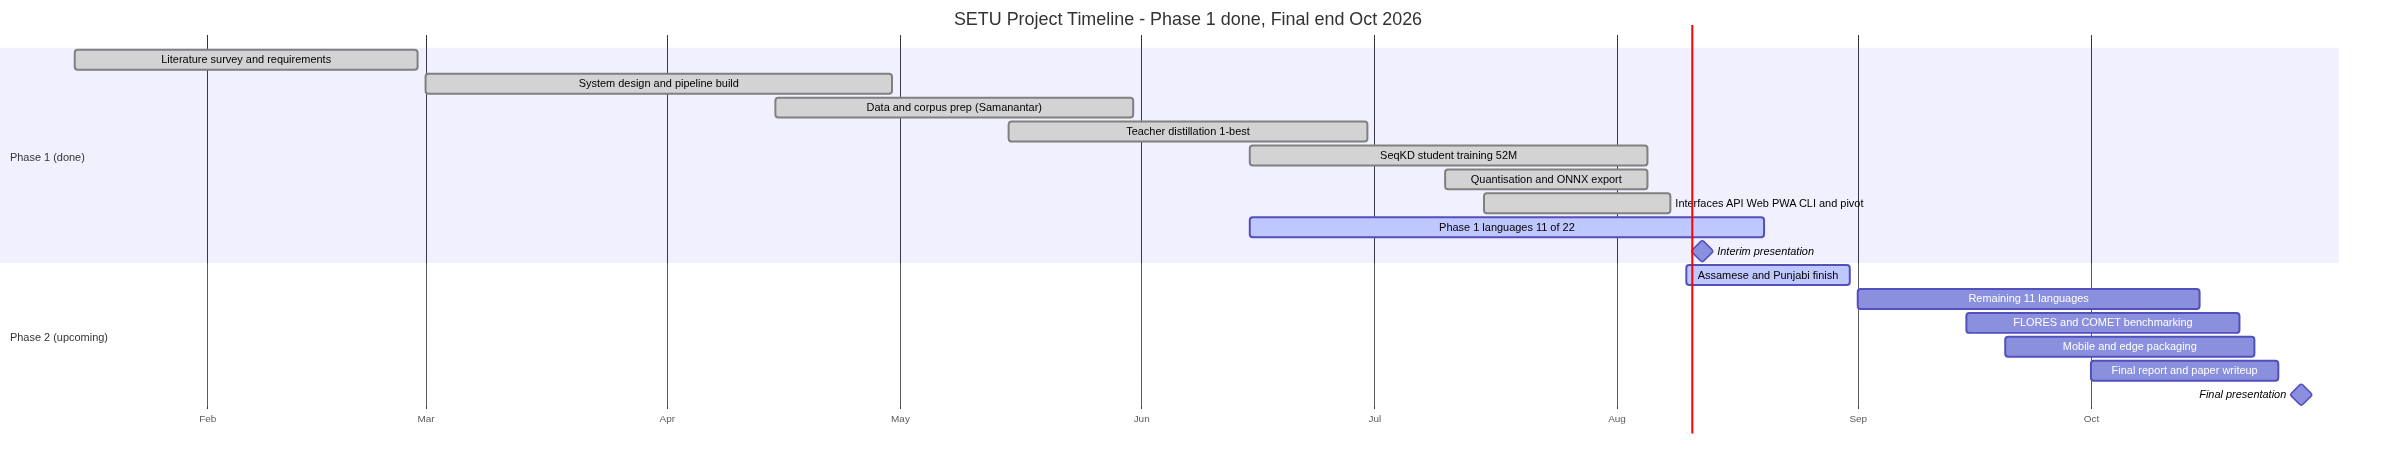
\includegraphics[width=0.99\textwidth, height=0.72\textheight, keepaspectratio]{figures/gantt.png}
\caption{Gantt chart --- Phase 1 complete, Phase 2 to the final presentation}
\label{fig:gantt}
\end{figure}

\begin{longtable}{@{}L{5.4cm} L{2.4cm} L{2.4cm} C{1.3cm} L{2.0cm}@{}}
\caption{Schedule of activities with durations}
\label{tab:schedule}\\
\toprule
\rowcolor{headblue}
\textbf{Activity} & \textbf{Start} & \textbf{Finish} & \textbf{Weeks} & \textbf{Status} \\
\midrule
\endfirsthead
\toprule
\rowcolor{headblue}
\textbf{Activity} & \textbf{Start} & \textbf{Finish} & \textbf{Weeks} & \textbf{Status} \\
\midrule
\endhead
\bottomrule
\endlastfoot

\multicolumn{5}{@{}l}{\textbf{Phase 1}}\\
Literature survey and requirements     & 15 Jan 2026 & 28 Feb 2026 & 6.5 & Complete \\
\rowcolor{rowgrey}
System design and pipeline build       & 01 Mar 2026 & 30 Apr 2026 & 8.5 & Complete \\
Corpus preparation (Samanantar)        & 15 Apr 2026 & 31 May 2026 & 6.5 & Complete \\
\rowcolor{rowgrey}
Teacher distillation (one-best)        & 15 May 2026 & 30 Jun 2026 & 6.5 & Complete \\
\seqkd{} student training (52\,M)      & 15 Jun 2026 & 05 Aug 2026 & 7.0 & Complete \\
\rowcolor{rowgrey}
Quantisation and ONNX export           & 10 Jul 2026 & 05 Aug 2026 & 3.5 & Complete \\
Interfaces: API, web, PWA, CLI, pivot  & 15 Jul 2026 & 08 Aug 2026 & 3.5 & Complete \\
\rowcolor{rowgrey}
Phase 1 language coverage (11 of 22)   & 15 Jun 2026 & 20 Aug 2026 & 9.5 & Complete \\
\textit{Interim presentation}          & \multicolumn{2}{l}{\textit{12 Aug 2026}} & --- & Milestone \\
\midrule
\multicolumn{5}{@{}l}{\textbf{Phase 2}}\\
\rowcolor{rowgrey}
Assamese and Punjabi completion        & 10 Aug 2026 & 31 Aug 2026 & 3.0 & Complete \\
Remaining 11 languages                 & 01 Sep 2026 & 15 Oct 2026 & 6.5 & In progress \\
\rowcolor{rowgrey}
FLORES-200 and COMET benchmarking      & 15 Sep 2026 & 20 Oct 2026 & 5.0 & In progress \\
Mobile and edge packaging              & 20 Sep 2026 & 22 Oct 2026 & 4.5 & Planned \\
\rowcolor{rowgrey}
Final report and paper write-up        & 01 Oct 2026 & 25 Oct 2026 & 3.5 & In progress \\
\textit{Final presentation}            & \multicolumn{2}{l}{\textit{28 Oct 2026}} & --- & Milestone \\

\end{longtable}

\subsection{PERT Analysis}
\label{subsec:pert}

The Programme Evaluation and Review Technique was applied to the Phase~1
activities, whose durations were genuinely uncertain. For each activity an
optimistic ($a$), most likely ($m$) and pessimistic ($b$) duration in weeks was
estimated, and the expected duration computed as

\begin{equation}
t_e = \frac{a + 4m + b}{6}, \qquad
\sigma = \frac{b - a}{6}, \qquad
\sigma^2 = \left(\frac{b-a}{6}\right)^{\!2}.
\end{equation}

\begin{table}[H]
\centering
\caption{PERT duration estimates for Phase 1 activities (weeks)}
\label{tab:pert}
\begin{tabular}{@{}c L{4.6cm} c c c c c c@{}}
\toprule
\rowcolor{headblue}
\textbf{ID} & \textbf{Activity} & \textbf{Pred.} & \textbf{$a$} & \textbf{$m$} & \textbf{$b$} & \textbf{$t_e$} & \textbf{$\sigma^2$} \\
\midrule
A & Literature survey \& requirements & ---    & 4 & 6  & 9  & 6.17  & 0.69 \\
\rowcolor{rowgrey}
B & System design                     & A      & 3 & 4  & 7  & 4.33  & 0.44 \\
C & Pipeline implementation (M0--M4)  & B      & 6 & 8  & 13 & 8.50  & 1.36 \\
\rowcolor{rowgrey}
D & Corpus preparation                & B      & 3 & 4  & 8  & 4.50  & 0.69 \\
E & Teacher distillation              & C, D   & 4 & 6  & 10 & 6.33  & 1.00 \\
\rowcolor{rowgrey}
F & Student training (\seqkd{})       & E      & 5 & 7  & 12 & 7.50  & 1.36 \\
G & Collapse diagnosis \& retraining  & F      & 0 & 2  & 5  & 2.17  & 0.69 \\
\rowcolor{rowgrey}
H & Quantisation \& ONNX export       & F      & 2 & 3  & 5  & 3.17  & 0.25 \\
I & Interfaces \& pivot routing       & H      & 2 & 3  & 6  & 3.33  & 0.44 \\
\rowcolor{rowgrey}
J & Evaluation \& scorecard           & G, H   & 1 & 2  & 4  & 2.17  & 0.25 \\
K & Documentation \& report           & I, J   & 2 & 3  & 5  & 3.17  & 0.25 \\
\bottomrule
\end{tabular}
\end{table}

Figure~\ref{fig:pert} shows the activity network. The critical path is
\textbf{A \arrowto{} B \arrowto{} C \arrowto{} E \arrowto{} F \arrowto{} G
\arrowto{} J \arrowto{} K}, with an expected duration of

\[
6.17 + 4.33 + 8.50 + 6.33 + 7.50 + 2.17 + 2.17 + 3.17 = \mathbf{40.34 \text{ weeks}},
\]

and a variance of $0.69+0.44+1.36+1.00+1.36+0.69+0.25+0.25 = 6.04$, giving a
standard deviation of $\sigma = 2.46$ weeks. Corpus preparation (D) and the
interface work (I) carry float and were not critical; the interface work was
deliberately scheduled in parallel with training so that a training delay would
not idle the team.

The analysis identifies student training (F) and the unplanned collapse
diagnosis (G) as the dominant risks, jointly contributing a third of the total
variance. This proved accurate: the two collapses described in
Section~\ref{sec:collapse} consumed almost exactly the two weeks that activity G
was allotted.

\begin{figure}[H]
\centering
\scalebox{0.92}{%
\begin{tikzpicture}[node distance=11mm and 13mm]
  \tikzset{ev/.style={circle, draw=black!75, fill=blue!5, minimum size=8.5mm,
                      font=\footnotesize, inner sep=0pt},
            crit/.style={-{Stealth[length=2.2mm]}, draw=red!70!black, very thick,
                         font=\scriptsize},
            norm/.style={-{Stealth[length=2mm]}, draw=black!65, font=\scriptsize}}
  % --- row 1: events 1..5 -------------------------------------------------
  \node[ev] (n1) {1};
  \node[ev, right=of n1] (n2) {2};
  \node[ev, right=of n2] (n3) {3};
  \node[ev, right=of n3] (n4) {4};
  \node[ev, right=of n4] (n5) {5};
  \node[ev, below=12mm of n3] (nd) {D};
  \draw[crit] (n1) -- node[above]{A} node[below]{6.17} (n2);
  \draw[crit] (n2) -- node[above]{B} node[below]{4.33} (n3);
  \draw[crit] (n3) -- node[above]{C} node[below]{8.50} (n4);
  \draw[crit] (n4) -- node[above]{E} node[below]{6.33} (n5);
  \draw[norm] (n3) -- node[right, pos=0.45]{D \ 4.50} (nd);
  \draw[norm] (nd) -| (n4);

  % --- row 2: events 5..8 and the finish ----------------------------------
  \node[ev, below=26mm of n1] (m5) {5};
  \node[ev, right=of m5] (m6) {6};
  \node[ev, right=of m6] (m7) {7};
  \node[ev, right=of m7] (m8) {8};
  \node[ev, right=of m8] (mf) {F};
  \node[ev, below=12mm of m6] (ni) {I};
  \draw[crit] (m5) -- node[above]{F} node[below]{7.50} (m6);
  \draw[crit] (m6) -- node[above]{G} node[below]{2.17} (m7);
  \draw[crit] (m7) -- node[above]{J} node[below]{2.17} (m8);
  \draw[crit] (m8) -- node[above]{K} node[below]{3.17} (mf);
  \draw[norm] (m6) -- node[right, pos=0.45]{H \ 3.17} (ni);
  \draw[norm] (ni) -| node[pos=0.22, below, font=\scriptsize]{I \ 3.33} (m8);
  \node[right=3mm of mf, font=\scriptsize] {finish};

  % row-continuation marker
  \draw[crit, dashed] (n5.south) .. controls +(0,-8mm) and +(0,8mm) .. (m5.north);
  \node[font=\scriptsize\itshape, black!60, right=1mm of n5] {continues below};

  \node[font=\scriptsize, align=left, below=9mm of ni, xshift=6mm]
       {\textcolor{red!70!black}{\rule{6mm}{1.2pt}} \ critical path: 40.34 weeks, $\sigma = 2.46$\\
        \textcolor{black!65}{\rule{6mm}{0.6pt}} \ non-critical activity (has float)};
\end{tikzpicture}}
\caption{PERT network for Phase 1 with the critical path highlighted}
\label{fig:pert}
\end{figure}

\subsection{Risk Management}
\label{subsec:risk}

Table~\ref{tab:risk} records the risks identified at planning time, together
with the mitigation applied and --- where the risk materialised --- what
actually happened. Five of the nine anticipated risks occurred.

\begin{longtable}{@{}p{1.0cm} L{3.5cm} C{1.3cm} C{1.3cm} L{6.0cm}@{}}
\caption{Risk register with outcomes}
\label{tab:risk}\\
\toprule
\rowcolor{headblue}
\textbf{ID} & \textbf{Risk} & \textbf{Prob.} & \textbf{Impact} & \textbf{Mitigation and outcome} \\
\midrule
\endfirsthead
\toprule
\rowcolor{headblue}
\textbf{ID} & \textbf{Risk} & \textbf{Prob.} & \textbf{Impact} & \textbf{Mitigation and outcome} \\
\midrule
\endhead
\bottomrule
\endlastfoot

R1 & Gated access to the teacher checkpoints and the BPCC corpus & High & High & Fall back to ungated rotary checkpoints and the Samanantar corpus. \textbf{Occurred.} Mitigation applied; the cost is a lower quality ceiling, reported explicitly \\
\rowcolor{rowgrey}
R2 & No GPU available locally & High & High & Use a cloud GPU (Kaggle, Colab) and later a dedicated A40 VM. \textbf{Occurred.} All final training ran on the A40 VM \\
R3 & Student fails to reach the quality target & Medium & High & Treat data volume, teacher strength and student width as independent levers; report shortfall honestly. \textbf{Partially occurred:} 14 of 22 directions pass \\
\rowcolor{rowgrey}
R4 & Training instability or divergence & Medium & High & Gradient clipping, learning-rate warmup, label smoothing; monitor training loss as a collapse indicator. \textbf{Occurred twice}; both recovered (Section~\ref{sec:collapse}) \\
R5 & Cloud session time limits kill long runs & High & Medium & Resumable runners with per-stage completion markers; persist artifacts outside the session. \textbf{Occurred} on Kaggle's 12-hour cap; resumability absorbed it \\
\rowcolor{rowgrey}
R6 & Quantised model exceeds the size budget & Low & High & Progressive INT8 then INT4 with per-stage measurement. \textbf{Did not occur:} 103.9\,MB against a 200\,MB budget \\
R7 & Inference too slow on CPU & Medium & High & ONNX Runtime with greedy decoding at deployment; beam search only offline. \textbf{Did not occur:} mean 105--202\,ms \\
\rowcolor{rowgrey}
R8 & Dependency and environment conflicts & Medium & Medium & Pin versions; audit the environment before each run. \textbf{Occurred} four times on the VM (Section~\ref{subsec:sw}); each fix folded into the runner \\
R9 & Insufficient corpus for low-resource languages & High & Medium & Prioritise languages with ungated data; document the blocked ones. \textbf{Occurred:} 11 of 22 languages delivered \\

\end{longtable}

\subsection{Team Organisation and Responsibilities}
\label{subsec:team}

The team of four divided the work by pipeline stage, with every member
responsible for the tests covering their own modules. Integration was
continuous: a milestone was not considered closed until the full test suite
passed, which forced interfaces to be agreed early rather than reconciled late.

\begin{table}[H]
\centering
\caption{Division of responsibility}
\label{tab:team}
\begin{tabular}{@{}L{3.3cm} L{2.4cm} L{8.2cm}@{}}
\toprule
\rowcolor{headblue}
\textbf{Member} & \textbf{USN} & \textbf{Primary responsibility} \\
\midrule
Jannat Zafrin & 1BI23AI017 & Literature survey; corpus pipeline (loading, normalisation, filtering, deduplication); evaluation harness and scorecard generation \\
\rowcolor{rowgrey}
Prabhav Sharma & 1BI23AI040 & Teacher integration and the abstraction wall; preference generation ($k$-NN retrieval, chrF ranking, validation); DPO trainer \\
Rishabh Sharma & 1BI23AI047 & \seqkd{} distiller and student trainer; GPU training campaign and runners; quantisation and ONNX export; collapse diagnosis and recovery \\
\rowcolor{rowgrey}
Sindhuja Tiwari & 1BI23AI054 & Inference engine and pivot router; REST API; Next.js client and offline PWA; CLI; test suite and documentation \\
\bottomrule
\end{tabular}
\end{table}

All four members contributed to system design, to the analysis of experimental
results, and to this report. Weekly review meetings with the guide governed
milestone closure, and the project log maintained in the repository records a
dated entry for every working session, which is the source from which
Chapter~\ref{ch:results} is reconstructed.
